\section{Comparison with HL-LHC PDF projections}
\label{app:comparisons_with_HLLHC}

%%%%%%%%%%%%%%%%%%%%%%%%%%%%%%%%%%%%%%%%%%%%%%%%%%%%%%%%%%%%%%%%%%%%%%%%
\begin{figure*}[!h]
	\centering
	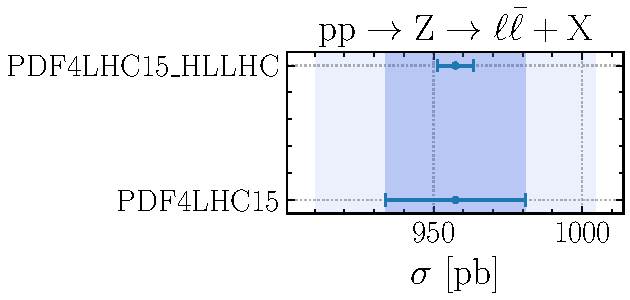
\includegraphics[width=0.32\textwidth]{plots/LHCpheno/NNPDF_DY_14TEV_40_PHENO-integrated-HLLHC.pdf}
	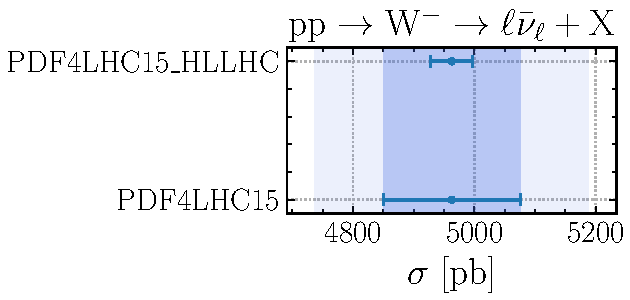
\includegraphics[width=0.32\textwidth]{plots/LHCpheno/NNPDF_WM_14TEV_40_PHENO-integrated-HLLHC.pdf}
	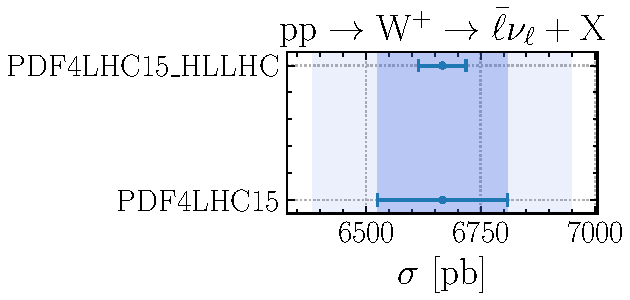
\includegraphics[width=0.32\textwidth]{plots/LHCpheno/NNPDF_WP_14TEV_40_PHENO-integrated-HLLHC.pdf}
	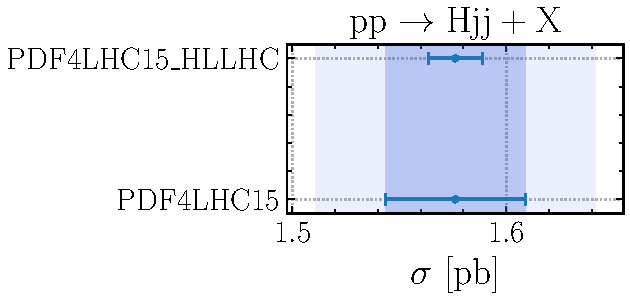
\includegraphics[width=0.32\textwidth]{plots/LHCpheno/NNPDF_HVBF_14TEV_40_PHENO-integrated-HLLHC.pdf}
	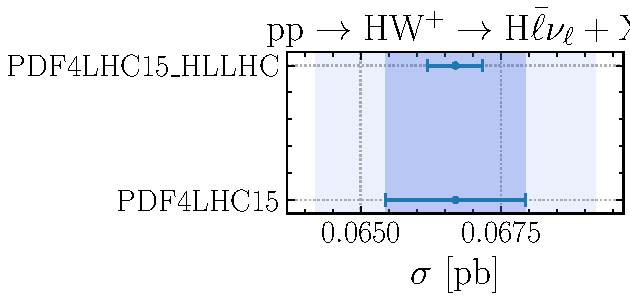
\includegraphics[width=0.32\textwidth]{plots/LHCpheno/NNPDF_HWP_14TEV_40_PHENO-integrated-HLLHC.pdf}
	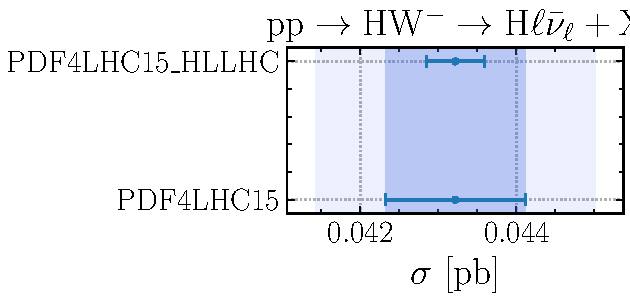
\includegraphics[width=0.32\textwidth]{plots/LHCpheno/NNPDF_HWM_14TEV_40_PHENO-integrated-HLLHC.pdf}
	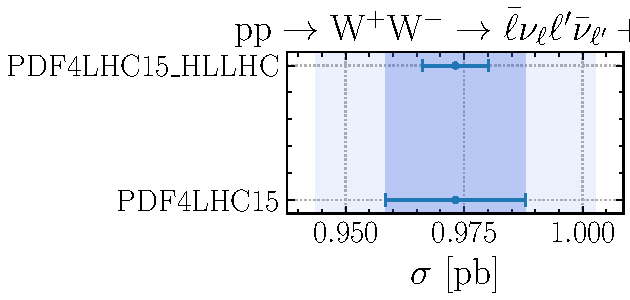
\includegraphics[width=0.32\textwidth]{plots/LHCpheno/NNPDF_WPWM_14TEV_40_PHENO-integrated-HLLHC.pdf}
	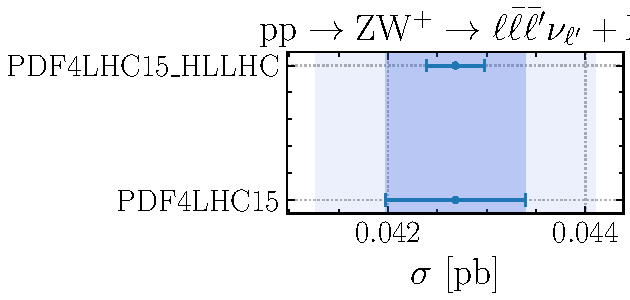
\includegraphics[width=0.32\textwidth]{plots/LHCpheno/NNPDF_WPZ_14TEV_40_PHENO-integrated-HLLHC.pdf}
	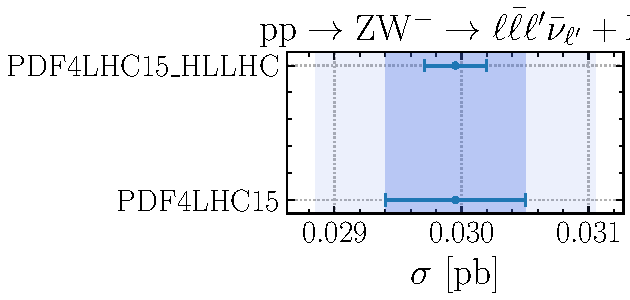
\includegraphics[width=0.32\textwidth]{plots/LHCpheno/NNPDF_WMZ_14TEV_40_PHENO-integrated-HLLHC.pdf}
	\caption{The same LHC fiducial cross-sections as in Fig.~\ref{fig:NNPDF40_pheno_integrated},
          now comparing the PDF4LHC15 baseline predictions with those based
          on the PDFs including HL-LHC pseudo-data from~\cite{AbdulKhalek:2018rok}.
          %
          Specifically, we consider the HL-LHC PDF projections
          from ``Scenario B'', corresponding to an intermediate scenario for the expected reduction
          of systematic uncertainties. }
	\label{fig:HLLHC_pheno_integrated}
\end{figure*}
%%%%%%%%%%%%%%%%%%%%%%%%%%%%%%%%%%%%%%%%%%%%%%%%%%%%%%%%%%%%%%%%%%%%%%%%

Here we revisit the phenomenology studies of
Sect.~\ref{sec:pheno} using the HL-LHC PDF impact projections
presented in~\cite{AbdulKhalek:2018rok}.
%
These projections were obtained with the same Hessian profiling strategy
as discussed in Sect.~\ref{sec:dis_pseudodata}, with the important
difference that the prior PDF set was PDf4LHC15 rather than
PDF4LHC21.
%
Therefore, while a direct comparison with the results presented in
Sect.~\ref{sec:pheno} is not possible due to the use of a different prior,
we can assess the relative reduction of PDF uncertainties in both cases,
and hence compare the reach on the PDFs of the FPF neutrino structure functions
and that of the HL-LHC measurements considered in the analysis of~\cite{AbdulKhalek:2018rok}.

This comparison of the relative PDF sensitivity of the FPF and
the HL-LHC data is interesting given that the  constraints from the 
two experiments are fully orthogonal and arise from completely different
scattering process.
%
Furthermore, the FPF constraints benefit from the valuable property
that an eventual contamination from new physics on the PDF fits 
can be neglected, since this process is driven by $Q^2$ values outside 
the possible presence of BSM physics (at least concerning new heavy particles).
%
Specially, should anomalies be revealed at the HL-LHC, having the independent
validation of the large-$x$ PDFs provided by the FPF would be extremely valuable 
for its interpretation.

Fig.~\ref{fig:HLLHC_pheno_integrated} displays the
same LHC fiducial cross-sections as in Fig.~\ref{fig:NNPDF40_pheno_integrated},
now comparing the PDF4LHC15 baseline predictions with those based
on the PDFs including HL-LHC pseudo-data from~\cite{AbdulKhalek:2018rok}.
%
Specifically, we consider the HL-LHC PDF projections
from ``Scenario B'', corresponding to an intermediate scenario for the expected reduction
of systematic uncertainties.
%
In general, the relative reduction on PDF uncertainties provided by the HL-LHC experiments
is more marked as in the case of the FPF pseudo-data, with the important caveat that
PDF4LHC21 already includes much more LHC data in comparison with its predecessor,
PDF4LHC15.
%
Another possible limiting assumption used in~\cite{AbdulKhalek:2018rok} is that
correlated uncertainties can be reliable estimated at the few-permille level
relevant for the intepretation of the HL-LHC data, something that is proving quite challenging
even for Run I and II measurements.

Nevertheless, the message obtained by comparing Fig.~\ref{fig:HLLHC_pheno_integrated} 
 with Fig.~\ref{fig:NNPDF40_pheno_integrated} is that of complementarity,
with the ultimate sensitivity on high-precision observables being
obtained by integrating the constraints both from the HL-LHC and from the FPF
in the same global determination of PDFs.


